\documentclass{swfcthesis}

\setlength{\arrayrulewidth}{0.5mm}

\addbibresource{thesis.bib}

\begin{document}

\Title{RongOS --- 简单操作系统的实现}
\Author{蒲启元}
\Advisor{王晓林}
\AdvisorTitle{讲师}
\AdvisorInfo{王晓林,男,49岁,硕士,讲师,毕业于英国格林尼治大学,分布式系统专业,现
  任西南林业大学计信学院教师,执教Linux、操作系统、网络技术等方面的课程,有丰富的Linux教学
  和系统管理经验。}
\Month{六}
\Year{二〇一八}

\Subject{计算机科学与技术专业} %专业名称(比如 电子信息工程专业)

\Abstract{操作系统管理着计算机的硬件和软件资源,它是向上层应用软件提供服务(接口)的核心系
  统软件,这些服务包括进程管理,内存管理,文件系统,网络通信,安全机制等。操作系统的设计与
  实现则是软件工业的基础。为此,在国务院提出的《中国制造2025》中专门强调了操作系统的开
  发\cite{china_2025}。但长期以来,操作系统核心开发技术都掌握在外国人手中,技术受制,对于我
  们的软件工业来说很不利。本项目从零开始设计开发个简单的操作系统,包括boot loader,中断,内
  存管理,图形接口,多任务,以及在这个系统上的几个小应用等。尽管这个系统很简单,但它为自主
  开发操作系统做了尝试。}

\Keywords{操作系统,进程,内存,中断,boot loader}

\Acknowledgments{首先我想感谢我的老师,王晓林。大学期间,他给了我很多指导,包括专业方面和上
  大学的意义等。很多时候,他对学生的要求看起来都是不近情理的,但正是通过这个“痛苦”的过程,
  我锻炼了坚强的意志,和战胜困难的信心。谢谢你,王老师。我最想感谢的是我的女友,她容忍我在
  完成这个设计时的很多个夜晚不陪她,给我支持,鼓励我,不抱怨。所以我愿意把这个简单操作系统
  命名为RongOS, 蓉便是她名字的最后一个字。谢谢你,我最亲爱的。}

\enTitle{RongOS --- A simple OS implementation}

\enAuthor{Qiyuan Pu}

\enAbstract{Operating system manages the resources of hardware and software, it lies
  in the core of the system software and provides services (interfaces) to upper
  applications. These services include process management, memory management, file system,
  network communication, security mechanism and more. Operating system development is the
  foundation and core of software industry. Therefore, \emph{Made in China
    2025} emphasizes the development of operating system that put forward by The State
  Council of China. For a long time, however, the OS kernel development technology is mastered
  by foreigner, due to technical limitations it is detrimental to our software industry. So this project will design and develop a simple operating system, including
  boot loader, interrupt, memory management, graphic interface, multitasking, and some
  little applications based on this system. In spite of the simplicity of this system,
  it's a small trying for autonomous development operating system.}

\enKeywords{operating system, boot loader, process, interrupt, memory management}

%%% 下面六行不要动!
\makepreliminarypages% 封面
\frontmatter          
\tableofcontents     % 目录
\listoffigures       % 插图目录
\listoftables        % 表格目录
\listoffixmes

\mainmatter

\chapter{Introduction}

\section{Background}
\label{sec:background}

Contemporary software systems are beset by problems that create challenges and
opportunities for broad new OS research. There are five areas could improve user
experience including dependability, security, system configuration, system extension, and
multiprocessor programming.

The products of forty years of OS research are sitting in everyone's desktop
computer, cell phone, car, etc., and it is not a pretty picture.
Modern software systems are broadly speaking complex, insecure, unpredictable, prone to
failure, hard to use, and difficult to maintain. Part of the difficult is that good
software is hard to write, but in the past decade, this problem and more specific
shortcomings in systems have been greatly exacerbated by increased networking and embedded
systems, which placed new demands that existing architectures struggled to meet. These
problems will not have simple solutions, but the changes must be pervasive, starting at
the bottom of the software stack, in the operating system.

The world needs broad operating system research. Dependability, security, system
configuration, system extension, and multi-processor programming
illustrate areas were contemporary operating systems have failed to meet the software
challenges of the modern computing environment\fxerror{\textbackslash{}cite\{hunt2005broad\}}.

\fxnote*{use citation instead, see \texttt{thesis.bib}}{Please reference.}


\section{Preliminary Works}

\subsection{Development Environment}
\label{sec:devel-envir}

\begin{description}
\item[OS platform:] Debian 9, Linux kernel 4.12.0-1-amd64
\item[Editor:] GNU Emacs 25.2.2
\item[Run time VM:] QEMU emulator 2.8.1
\item[Assembler:] Nask
\item[Compiler:] CC1(Based on gcc)
\item[Debugger:] \fxnote{debugger?}
\end{description}

\subsection{Tools}
\label{sec:tools}

Some tools were used to develop RongOS, \xout{see tools}\fxerror{need some descriptions about
  the tools}\footnote{\url{https://github.com/Puqiyuan/RongOS/tree/master/Tools}}. Note
that these tools are Windows executables \fxerror{(so what?)}\xout{exe format based on
  Windows system}. Among these tools, the most important ones are:

\begin{description}
\item[nask.exe] the assembler, a modified version of NASM
\item[cc1] the C compiler
\end{description}

\subsection{Platform Setup}
\label{sec:install}

The development platform (mainly the Debian system) was setup by following the
\emph{Debian Installation
  tutorial}\footnote{\url{http://cs2.swfc.edu.cn/~wx672/lecture_notes/linux/install.html}}. The
main steps were:
\begin{enumerate}
\item Installing the base system;
\item Installing necessary software tools, such as emacs, web browser, qemu, wine, etc.;
\item Cloning configuration files by following the tutorial;
\item Some more miscellaneous tweaks to satisfy my personal needs.
\end{enumerate}

\xout{Debian System: there is a small tutorial. This tutorial is a sample one for set up
  development environment, the main thing is operating system --- Debian.}

\subsubsection{Qemu}
\label{sec:qemu}

QEMU is a generic and open source machine emulator and virtualizer.\fxerror{need citation}
In this project, QEMU was used as the test bed.\xout{ to test the running result.}

Installing QEMU for my x86\_64 architecture is as easy as the following command: 
\begin{verbatim}
     $ sudo apt-get install qemu-system-x86_64
\end{verbatim}

\subsubsection{Wine}
\label{sec:wine}

Wine (originally an acronym for "Wine Is Not an Emulator") is a compatibility layer
capable of running Windows applications on several POSIX-compliant operating systems, such
as Linux, macOS, and BSD.\fxerror{need citation}

Because the tools I used in this project are in Windows exe format, so on Debian system,
Wine need to be installed:
\begin{verbatim}
     $ sudo apt-get update
     $ sudo apt-get install wine
\end{verbatim}

\subsubsection{Debian i386 support}
\label{sec:debian-i386-support}

On 64-bit systems you need to enable multiarch support 
for running 32-bit Windows applications (many modern apps are
still 32-bit, also for large parts of the Windows subsystem itself), our development
tools are 32-bit Windows applications, so add this architecture:

\begin{verbatim}
     $ sudo dpkg --add-architecture i386
     $ sudo apt-get update
\end{verbatim}

\chapter{Leading Knowledge}
\label{cha:leading-knowledge}

\label{cha:leading-knowledge-1}

\section{Mouse}
\label{sec:mouse}

\section{The Leap --- Road to the 32 Bit Mode}
\label{sec:leap-road-32}



\section{Data Structure}
\label{sec:data-structure}
\fxerror{Data Structure}

\section{Programmable Interrupt Controller}
\label{sec:progr-interr-contr}

\fxerror{Programmable interrupt controller}

\section{C Language Basis}
\label{sec:c-language-basis}
\fxerror{C language basis}

\section{Segment and Descriptor}
\label{sec:segment-descriptor}
\fxerror{segment and}


\section{Instruction Set}
\label{sec:instruction-set}

An instruction set architecture (ISA) is an abstract model of a computer. It is also
referred to as architecture or computer architecture. An ISA defines everything a machine
language programmer needs to know in order to program a computer.

An ISA may be classified in a number of different ways. A common classification is by
architectural complexity. A complex instruction set computer (CISC) has many specialized
instructions, some of which may only be rarely used in practical programs. A reduced
instruction set computer (RISC) simplifies the processor by efficiently implementing only
the instructions that are frequently used in programs, while the less common operations
are implemented as subroutines, having their resulting additional processor execution time
offset by infrequent use.

On traditional architectures, an instruction includes an opcode that specifies the
operation to perform, such as add contents of memory to register—and zero or more operand
specifiers, which may specify registers, memory locations, or literal
data\fxerror{\textbackslash{}cite\{...\}}.

\xout{Please reference} \fxerror{use citation rather than footnote}%\footnote{\url{https://en.wikipedia.org/wiki/Instruction_set_architecture}}.

The simple RongOS is based on x86 architecture, the following instructions are common
for RongOS:

\begin{description}
\item[db:] the abbreviation of define byte, write a byte, also 8 bits to file.
\item[resb:] the abbreviation of reserve byte, reserved bytes and filling 0x00 in these reserved space.
\item[dw:] the abbreviation of define word, write two bytes, also 16 bits to file.
\item[dd:] the abbreviation of define double-word, write four bytes, also 32 bits to file.
\item[org:] load the program to specified address.
\item[jmp:] jump to another instruction.
\item[mov:] assign the right value to left variable.
\item[jc:] the abbreviation of jump if carry, it means if carry flag is 1, jump.
\item[jnc:] jump if not carry.
\item[jae:] jump if above or equal.
\item[jbe:] jump if below or equal.
\item[jb:] jump if below.
\item[equ:] equ is the abbreviation of equal.
\item[ret:] end of function, return.
\item[in:] get signal from device.
\item[out:] send signal to device.
\item[cli:] clear interrupt flag, set it to 0.
\item[sti:] set interrupt flag, set it to 1.
\item[pushfd:] push flags double-word
\item[popfd:] pop flags double-word
\item[lgdt:] load content from specified memory to initialize GDT(global descriptor table)
  register.
\item[lidt:] load content from specified memory to initialize IDT(interrupt descriptor
  table) register.
\end{description}

\section{x86 Registers}
\label{sec:register}

In computer architecture, a processor register is a quick accessible location available
to a computer's central processing unit (CPU). Registers usually consist of a small amount
of fast storage, although some registers have specific hardware functions, and may be
read-only or write-only.  Almost all computers, whether load/store architecture or not,
load data from a larger memory into registers where it is used for arithmetic operations
and is manipulated or tested by machine instructions. Manipulated data is then often
stored back to main memory, either by the same instruction or by a subsequent one. Modern
processors use either static or dynamic RAM as main memory, with the latter usually
accessed via one or more cache levels.\fxerror{need citation}

Processor registers are normally at the top of the memory hierarchy, and provide the
fastest way to access data. The term normally refers only to the group of registers that
are directly encoded as part of an instruction, as defined by the instruction
set. Registers are normally measured by the number of bits they can hold, for example, an
``8-bit register'' or a ``32-bit register''. For x86 architecture, the following registers
exist:

\begin{multicols}{3}
  \begin{description}
  \item[ax:] accumulator
  \item[bx:] base
  \item[cx:] counter
  \item[dx:] data
  \item[bl:] base low
  \item[al:] accumulator low
  \item[cl:] counter low
  \item[dl:] data low
  \item[bh:] base high
  \item[ah:] accumulator high
  \item[ch:] counter high
  \item[dh:] data high
  \item[sp:] stack pointer
  \item[bp:] base pointer
  \item[si:] source index
  \item[di:] destination index
  \item[es:] extra segment
  \item[cs:] code segment
  \item[ss:] stack segment
  \item[ds:] data segment
  \item[fs:] no name
    % \item[gs:] no name
  \end{description}
\end{multicols}

Among these registers, \fxnote*{better be \textbackslash{}texttt\{bx, bp, si\}}{bx, bp, si}
and di can be used to specify the address of memory. But ax, cx, dx and sp can not.  When
mov instruction is used\xout{using}, \fxerror*{don't understand.}{the number of bits of
  operation number should be the same}. 16-bit registers: ax, cx, dx, bx, sp, bp, si, di,
es, cs, ss, ds and fs. 8-bit registers: al, cl, dl, bl, ah, ch, dh and bh. Actually, all
these 8-bit registers are part of corresponding 16-bit registers, low 8 bits or high 8
bits.\fxnote{perhaps you can add a picture to illustrate your understanding.}

\section{Interrupt Call}
\label{sec:interrupted-call}

BIOS interrupt calls perform hardware control or I/O functions requested by a program,
return system information to the program, or do both\fxerror{need citation}. A key element
of the purpose of BIOS calls is abstraction. The BIOS calls perform generally defined
functions, and the specific details of how those functions are executed on the particular
hardware of the system are encapsulated in the BIOS and hidden from the program. The
interrupt calls are commonly used in RongOS are listed in Table~\ref{tbl:intcall}.

\begin{table}[!ht]
  \centering\tabulinesep=2mm
  \begin{tabu}{|X[c,m,-1]|X[l,m]|X[-1,l,m]|X[-1,c,m]|}
    \tabucline-
    Interrupt\par{}Number & Register Parameter & Return Value & Function\\ \tabucline-
    0x10 &
    ah=0x0e(write character in tty mode)\par{}
    al=character code\par{}
    bh=0, bl=colorcolor& null & video services \\\tabucline-
    0x13 &
    ah=0x02(read sectors)\par{}
    ah=0x03(write sectors)\par{}
    ah=0x04(verify sectors)\par{}
    ah=0x0c(seek to specified track)\par{}
    al=number of sectors processing\par{}
    ch=cylinder \& 0xff  cl=sector number\par{}
    dh=header number dl=driver number\par{}
    es:bx=buffer address &
    FLACS.CF=0\par{}
    no error, ah = 0\par{}
    FLAGS.CF=1\par{}
    error, ah=error number\par{}& disk services \\ \tabucline-
  \end{tabu}
  \caption{RongOS interrupt calls}\label{tbl:intcall}
\end{table}

\section{Memory Map}
\label{sec:memory-map}

In the boot process, a memory map is passed on from the firmware in order to instruct an
operating system kernel about memory layout\fxerror{need citation}. It contains the
information regarding the size of total memory, any reserved regions and may also provide
other details specific to the architecture. For loading RongOS to memory, the memory layout
should be clarified as in Table~\ref{tbl:memlayout}.

\begin{table}[!ht]
  \centering\tabulinesep=2mm
  \begin{tabu}{|c|c|c|c|} \tabucline-
    Range(in hexadecimal) & Range(in decimal) & Size(in bytes) & Usage \\
    \tabucline-
    0000 --- 03ff & 0000 --- 1023 & 1024 &  interrupt vector table \\
    \tabucline-
    0400 --- 04ff & 1024 --- 1279 & 256 & BIOS data area \\
    \tabucline-
    0500 --- 051f & 1280 --- 1311 & 32 & Reserved \\
    \tabucline-
    0520 --- 7bff & 1312 --- 31743 & 30432 & conventional memory  \\
    \tabucline-
    7c00 --- 7dff & 31744 --- 32255 & 512 & master boot record \\
    \tabucline-
    7e00 --- 9ffff & 32256 --- 655359 & 623104 & conventional memory \\
    \tabucline-
    a0000 --- affff & 655360 --- 720895 & 64K & VGA graphics RAM \\
    \tabucline-
    b0000 --- b7fff & 720896 --- 753663 & 32K & monochrome text mode \\
    \tabucline-
    b8000 --- bffff & 753664 --- 786431 & 32K & color text mode \\
    \tabucline-
    c0000 --- c7fff & 786432 --- 819199 & 32K & VGA video ROM \\
    \tabucline-
    c8000 --- cbfff & 819200 --- 835583 & 16K & IDE hard drive \\
    \tabucline-
    cc000 --- cffff & 835584 --- 851967 & 16K & optional adaper \\
    \tabucline-
  \end{tabu}
  \caption{RongOS Memory Layout}\label{tbl:memlayout}
\end{table}

\section{Floppy Disk}
\label{sec:floppy-disk}

There are many ways to boot an operating system, from hard disk, USB, floppy disk, etc.
The structure of floppy disk is simple and for this simple operating system, it's enough.

Fig.~\ref{fig:flpy1.png} shows the inside of a floppy disk:
\begin{figure}[!ht]
  \centering
  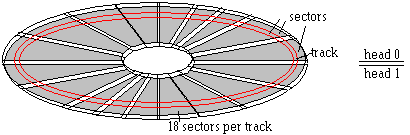
\includegraphics[width=.5\textwidth]{../figs/bootLoader/flpy1.png}
  \caption{Floppy Disk Structure}
  \label{fig:flpy1.png}
\end{figure}

A floppy disk, also called a floppy, diskette, or just disk, is a type of disk storage
composed of a disk of thin and flexible magnetic storage medium, sealed in a rectangular
plastic enclosure lined with fabric that removes dust particles. Floppy disks are read and
written by a floppy disk drive (FDD).\fxerror{need citation}

For 3.5 inch HD floppy,  There are 80 cylinders from the outermost to
the core on each side, numbering 0, 1, \ldots, 79. The head can assign be 0 or 1,
representing two sides of floppy. When specify head number and cylinder number, forming a
ring, named track in jargon. The track is large so we divide it to 18 small parts, named
sector. A sector can store 512 byte. So the capacity of a floppy is:

\[18 \times 80 \times 2 \times 512 = 1474560 Byte = 1440 KB\]


\chapter{Design}

\section{Top Level Design}
\label{sec:top-level-design}


\subsection{32-bit Mode and Import C Codes}
\label{sec:32-bit-mode}


\chapter{Implementation}

\section{Boot Loader}

\subsection{Flowchart of Boot Loader}
\label{sec:flowch-boot-load}

Fig.~\ref{fig:flowchart-of-boot-loader} shows how the boot loader works.

\begin{figure}[!ht]
  \centering
  % 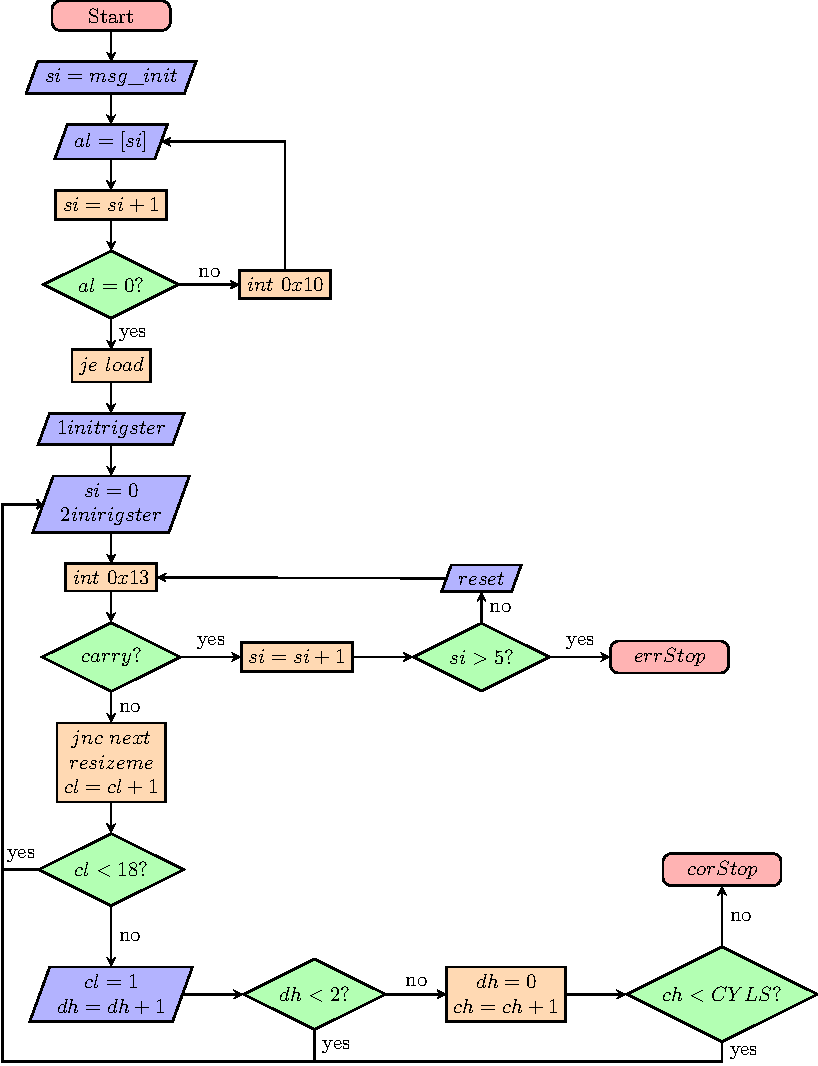
\includegraphics[width=1\textwidth]{../figs/FlowchartTex/1/flowcharte.pdf}
  \fxerror{need a better chart}
  \caption{Flowchart of Boot Loader}
  \label{fig:flowchart-of-boot-loader}
\end{figure}

The boot loader is implemented in Intel assembly. It works as following:

\fxerror{use \textbackslash{}texttt\{0x10,ax,al,...\}, rather than \$0x10,ax,al,...\$}
\begin{enumerate}
\item \textbf{Display boot information:} Firstly, the boot sector display some boot information,
  when $al=0$, the null character of boot information hit. Interrupt $0x10$ is used for
  show a character. Appendix ~\ref{sec:dis-boo-inf} is the code to perform this function.
\item \textbf{Read the second sector:} Then jump to load C0-H0-S2, $ax$ register saved the address
  where beginning puts the sectors from floppy. And preparing parameters for interrupt
  $0x13$ in registers. The $0x13$ interrupt used for read sector from floppy to
  memory. Appendix ~\ref{sec:rea-sec-sec} is the code to perform this function.
\item \textbf{Read two sides of a track:} If there is a carry, representing some thing wrong when
  read floppy, so reset the registers and try again read floppy, until five times
  trying. Register $si$ is a counter. If no carry, jump to next segmentation, as one
  sector read to memory already, the address space should increase 512 byte. Then sector
  number($cl$ register) added 1 and compare it to 18, if it's smaller than 18, jump to
  $readloop$, read the next sector. If the value of $cl$ register bigger or equal to than
  18, meaning that one track 18 sector in this side of floppy read already, then reversed
  the head, add 1 to $dh$ register. If the value of $dh$ register after adding larger than
  or equal to 2, it's saying the original head is 1, one track of two sides read
  already. Otherwise the value of $dh$ register smaller than 2, read this side indicating
  by $dh$ register, jump to $readloop$ segmentation. Appendix ~\ref{sec:rea-two-sid} is
  the code to perform this function.
\item \textbf{The next cylinder:} So the next step is moving a cylinder, add 1 to register
  $ch$. Otherwise the value of $dh$ register smaller than 2, read this side indicating by
  $dh$ register, jump to $readloop$ segmentation. After $ch$ register add 1, if it's
  smaller than 10, jump to $readloop$, otherwise end loading floppy to memory process, for
  we only load ten cylinders of floppy. Appendix ~\ref{sec:the-nex-cyl} is the code to
  perform this function.
\end{enumerate}

\subsection{Running Result}
\label{sec:running-result}

Fig.~\ref{fig:iplRes} shows the running results of boot loader. From this picture we
see that the boot loader loaded 10 cylinders from floppy successfully. 

\begin{figure}[!ht]
  \centering
  % 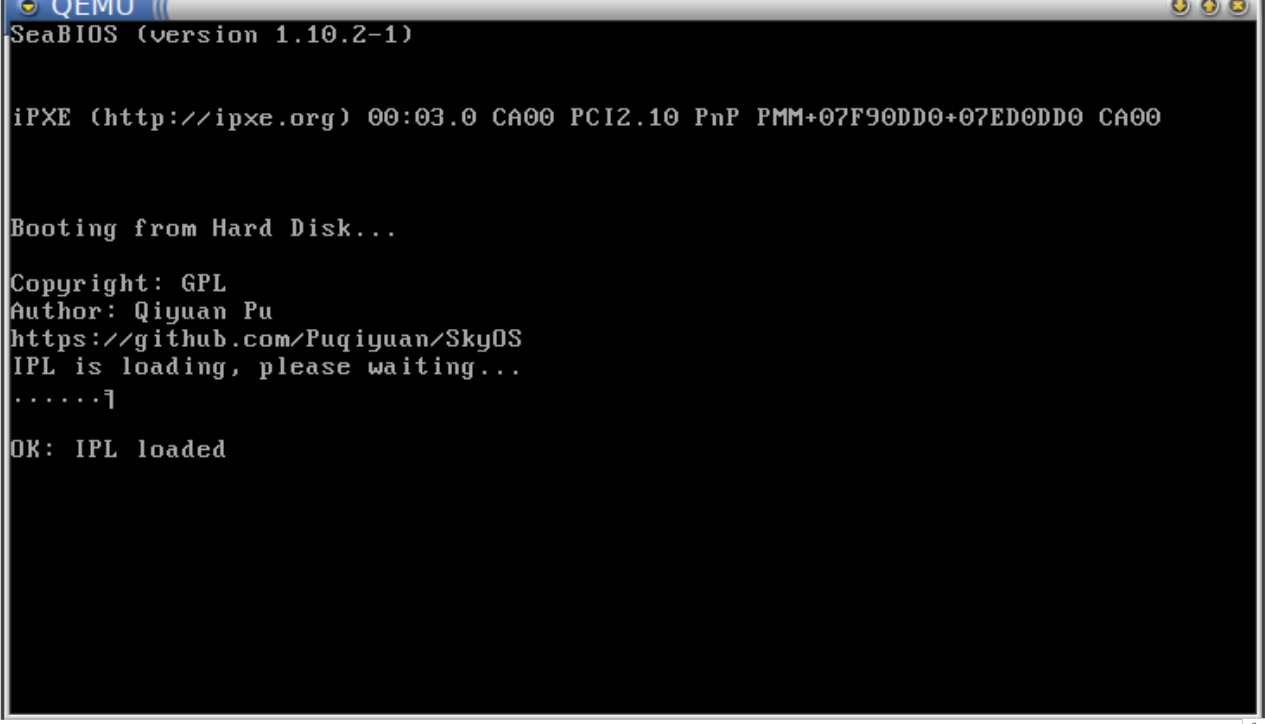
\includegraphics[width=1.1\textwidth]{iplRes.png}
  \fxerror{need a better pic.}
  \caption{Running Result of Boot Loader}
  \label{fig:iplRes}
\end{figure}



\section{32-bit Mode and Import C Codes}


\section{Screen Display and Text}

\section{Control Mouse}


\section{Memory Management}

\section{Making Window }

\section{Timer}

\section{Multitasking}

\section{Command Line Window}

\section{API}

\section{OS Protection}

\section{Graphics Processing}

\section{Window Operation}

\section{Application Protection}

\section{File Operation}

\section{Some Applications}

\chapter{Prospects And Shortages}

%%% 正文部分到此结束。下面是『参考文献』、『指导教师简介』、『鸣谢』、『附录』

%% 不要动下面四行!
\Appendix{}
\printbibliography[heading={bibintoc},title={参考文献}] % 输出参考文献
\advisorinfopage{}                 % 输出指导教师简介
\acknowledgmentspage{}             % 输出鸣谢

%%% 下面是附录部分,可以没有。

\chapter{Main Program Code} %附录一

\section{Boot loader}

\subsection{Display boot information}
\label{sec:dis-boo-inf}

\inputminted[firstline=55, lastline=65,
  linenos=true]{nasm}{../../src/06day/RongC/ipl10.asm}

\subsection{Read the second sector}
\label{sec:rea-sec-sec}
  
\inputminted[firstline=87,lastline=106,linenos=true]{nasm}{../../src/06day/RongC/ipl10.asm}

\subsection{Read two sides of a track}
\label{sec:rea-two-sid}

\inputminted[firstline=108,lastline=132,linenos=true]{nasm}{../../src/06day/RongC/ipl10.asm}

\subsection{The next cylinder}
\label{sec:the-nex-cyl}

\inputminted[firstline=134,lastline=137,linenos=true]{nasm}{../../src/06day/RongC/ipl10.asm}

\end{document} % 结束。不要动下面几行!

%%% Local Variables:
%%% mode: latex
%%% TeX-master: t
%%% End:
